% Load the base class
\documentclass[minted, draw]{../tex/hebdomon}
\usepackage{svg}
\usepackage{biblatex}[backend=biber, style=ieee, sorting=none]
\addbibresource{references.bib}
\begin{document}



\publishers{
  \begin{tabular}[!b]{rl}
  \textbf{Student Name} & Achille Cannavale \\[3pt]
  \textbf{Student Number} & xxxxx \\[3pt]
  \textbf{Module Name} & xxxxx
  \end{tabular}\\[20pt]
  }

\begin{titlepage}
    \centering
	
\includegraphics[width=4cm]{figures/logo.png}\par\vspace{1cm}

    %\vspace*{2cm}

    {\scshape\LARGE Università degli Studi di Cassino e del Lazio Meridionale\par}
    \vspace{1cm}
    {\Large Corso di Laurea Magistrale in Ingegneria Informatica \par}

    \vspace{2cm}
    {\Huge\bfseries Segmentazione del seno in immagini MRI\par}
    \vspace{1cm}
    {\large Versione 0.1}

    \vfill

    \begin{flushleft}
    \textbf{Studente}: Achille Cannavale \\
	\textbf{Matricola}: 59721 \\
    \textbf{Relatore}: Alessandro Bria \\
    \end{flushleft}

    \vspace{1.5cm}

    {\large \today\par}
\end{titlepage}

\dominitoc
\tableofcontents
\newpage




\Chapter{}
\Section{Introduzione}

La segmentazione di strutture anatomiche in immagini mediche 3D rappresenta un task importante nell’ambito clinico e diagnostico. In particolare la segmentazione del seno da immagini MRI (Magnetic Resonance Imaging) 3D è un task complesso, ma essenziale per applicazioni come la pianificazione di interventi chirugici o l’analisi di anomalie tessutali.

In passato, la segmentazione del seno in immagini MRI 3D veniva effettuata principalmente con \textbf{metodi classici}, spesso semi-automatici o manuali, basati su:

\begin{itemize}
	\item \hlight{Approcci a soglia} (thresholding) e \hlight{region-growing}, che sfruttavano differenze di intensità tra tessuti ma richiedevano regolazioni manuali e fallivano in presenza di rumore o basso contrasto.
	\item \hlight{Deformable models} (es.: Active Contours) e \hlight{algoritmi a clustering} (es.: k-means), sensibili all’inizializzazione e poco robusti alla variabilità anatomica.
	\item Metodi \hlight{atlas-based}, che allineavano immagini a template pre-annotati, limitati però dalla diversità inter-paziente.
\end{itemize}

Con l’avvento del \textbf{deep learning}, in particolar modo delle reti convoluzional e di architetture come \hlight{U-Net 3D}, la segmentazione del seno ha raggiunto livelli di accuratezza più alti rispetto al passato. 


\Section{Background e Stato dell'Arte}

La segmentazione semantica di immagini mediche rappresenta uno dei compiti fondamentali nell’ambito della diagnostica per immagini assistita da computer (CAD - Computer Aided Diagnosis). Essa consente di delineare strutture anatomiche e lesioni, migliorando l’accuratezza e l’efficienza dei processi diagnostici e terapeutici.

Negli ultimi anni, l'avvento del deep learning ha rivoluzionato il campo dell’elaborazione di immagini mediche, introducendo architetture sempre più sofisticate per la segmentazione automatica. Una delle architetture più note e utilizzate è la \textbf{U-Net}, proposta da Ronneberger et al. \cite{ronneberger2015unet}, che ha introdotto un design encoder-decoder con connessioni skip per preservare i dettagli spaziali durante il processo di ricostruzione dell'immagine segmentata.

Successivamente, sono state sviluppate numerose varianti e miglioramenti, tra cui architetture basate su reti convoluzionali più profonde, reti residuali e approcci multi-scala. Tuttavia, negli ultimi anni l’interesse si è spostato verso l’impiego di \textbf{Transformers}, inizialmente sviluppati per il Natural Language Processing (NLP), e adattati con successo al dominio delle immagini mediche. Esempi notevoli sono \textbf{TransUNet} \cite{chen2021transunet} e \textbf{Swin UNETR} \cite{hatamizadeh2022swin}, che combinano l’efficacia dei Transformers nel modellare le dipendenze globali con la capacità di apprendere rappresentazioni spaziali locali, tipiche delle CNN.

Il framework \textbf{MONAI} (Medical Open Network for AI) \cite{cardoso2022monai} si è affermato come uno standard de facto nello sviluppo di pipeline per la segmentazione e classificazione di immagini mediche. Basato su PyTorch, MONAI offre un’ampia gamma di trasformazioni, modelli predefiniti, reader DICOM e metriche di valutazione, risultando particolarmente adatto per workflow in ambito sanitario.

Nel presente lavoro, è stato impiegato MONAI per la gestione dei dati e la costruzione della pipeline di addestramento. Per il task di segmentazione della mammella su risonanza magnetica, si è fatto uso del dataset \textbf{Duke-Breast-Cancer-MRI}, disponibile su The Cancer Imaging Archive (TCIA) \cite{duke_breast_mri}, che contiene serie DICOM annotate manualmente da radiologi esperti.

\Section{Attività di Tirocinio}

L’attività si è inserita nel contesto di un progetto di ricerca mirato allo sviluppo e alla valutazione di modelli di segmentazione automatica per immagini di risonanza magnetica della mammella, con particolare attenzione.

L’obiettivo principale del tirocinio è stato quello di sperimentare e ottimizzare pipeline basate su \textbf{deep learning} per la segmentazione semantica tridimensionale, utilizzando framework open-source moderni come \textbf{MONAI} (Medical Open Network for AI) e \textbf{PyTorch}.

Le principali attività svolte durante il tirocinio sono state:
\begin{itemize}
    \item \textbf{Pre-processing} dei dati in formato DICOM, con conversione in formato leggibile da MONAI e normalizzazione dell’intensità del segnale.
    \item Composizione e validazione di un dataset bilanciato, con partizionamento in training, validation e test set.
    \item Studio e implementazione di modelli di segmentazione basati su architetture \textbf{state-of-the-art}, tra cui \textbf{UNet} e \textbf{AttentionUNet}.
    \item Configurazione degli esperimenti, tuning degli iperparametri e addestramento dei modelli in ambiente GPU.
    \item Valutazione delle prestazioni mediante metriche standard come Dice coefficient
\end{itemize}

Durante il tirocinio sono state inoltre affrontate e risolte diverse problematiche tecniche legate alla gestione dei metadati DICOM, alla compatibilità tra i formati di input, e alla gestione efficiente della memoria in fase di training. L'intero lavoro è stato documentato e riproducibile mediante script Python e configurazioni YAML modulari.




%
% \begin{figure}[ht]
% 	\centering
% 	\includesvg[width=\linewidth]{figures/pipeline_general.svg}
% 	\caption{Pipeline Generale del nostro progetto, suddivisa in una fase di Deep Learning per per la rilevazione delle ROI e l'estrazione delle features e una fase di Machine Learning per la classificazione delle cellule.}
% 	\label{fig:pipeline_general}
% \end{figure}

	
\Section{Strumenti Utilizzati}
Durante il tirocinio sono stati impiegati diversi strumenti software e librerie  fondamentali per la gestione, il pre-processing e l'elaborazione di immagini medicali, nonché per lo sviluppo e il training di modelli di deep learning.
\begin{itemize}
	\item  Il linguaggio principale di lavoro è stato \textbf{Python}, scelto per la sua flessibilità e per l'ampio ecosistema di librerie scientifiche.
	\item Per la manipolazione delle immagini DICOM è stata utilizzata la libreria \textbf{MONAI} (Medical Open Network for AI), un framework open-source basato su PyTorch e progettato specificamente per applicazioni di imaging medicale. MONAI ha permesso di gestire agevolmente il caricamento dei dati, le trasformazioni e la normalizzazione delle immagini, grazie a un sistema modulare di trasformazioni componibili.
	\item Il framework di deep learning impiegato è stato \textbf{PyTorch}, scelto per la sua semplicità d'uso, il supporto attivo della community e le sue prestazioni elevate, specialmente in combinazione con l'accelerazione GPU fornita da CUDA.
	\item Lo sviluppo del codice è stato realizzato su una macchina Linux, con accesso remoto e con l'ausilio dell'editor \textbf{Visual Studio Code}.
\end{itemize}













\Section{Composizione del Dataset}

Il dataset utilizzato durante il tirocinio proviene dal database \hlight{Duke Breast Cancer MRI}, un archivio pubblico contenente immagini DICOM di risonanze magnetiche della mammella. Ogni caso clinico è organizzato in una struttura gerarchica che riflette l'identificativo univoco del paziente e delle relative acquisizioni.

Il dataset è composto da sequenze \hlight{DICOM} tridimensionali, ciascuna rappresentante un'acquisizione volumetrica del seno. In tutti i casi sono disponibili anche annotazioni o maschere segmentate manualmente da esperti, utilizzate come ground truth per il training dei modelli di segmentazione.

Durante la fase di preparazione, le immagini sono state convertite in formato compatibile con MONAI tramite una pipeline di preprocessing, che ha incluso:
\begin{itemize}
    \item il \textbf{caricamento} delle immagini in memoria;
    \item la standardizzazione dell'intensità e il ridimensionamento spaziale;
    \item l'organizzazione dei dati in \textbf{dizionari} contenenti sia l'immagine sia i relativi metadati;
    \item la \textbf{salvataggio} del dataset preprocessato 
\end{itemize}

Per ogni volume è stata mantenuta l'associazione tra immagine e metadati (es. spacing, orientamento, posizione del paziente), necessari per garantire una corretta elaborazione e interpretazione dei dati durante le fasi di training, validazione e inferenza.

L'intero dataset è stato infine suddiviso in tre sottoinsiemi: \hlight{training}, \hlight{validation} e \hlight{test}, rispettando la proporzione e la varietà dei casi clinici per assicurare una valutazione affidabile delle performance del modello.



\Chapter{Deep Learning}

\Section{Trasformazioni}
Per garantire una buona generalizzazione del modello, sono state provate diverse trasformazioni, usando la libreria \hlight{Albumentation}, tra le quali sono state scelte le seguenti migliori per il nostro caso di studio: (anche una tabella va bene)


%
\begin{table}[!ht]
	\begin{NiceTabular}{rX}[rules/color=[gray]{0.9},rules/width=1pt]
		\CodeBefore
		\rowcolors{1}{black!5}{}
		\rowcolors{3}{blue!5}{}
		\Body
		\toprule
		\textbf{Trasformazione}      & \textbf{Parametri}                                \\
		\midrule
		\textbf{A.HorizontalFlip} & p=0.5          \\
		\textbf{A.VerticalFlip}   & p=0.5        \\
		\textbf{A.ColorJitter} & brightness=0.2, contrast=0.2, saturation=0.2, hue=0.1, p=0.3\\
		\textbf{A.RandomBrightnessContrast} & p=0.3\\
		\textbf{A.MotionBlur} & p=0.2\\
		\textbf{A.GaussNoise} & p=0.2\\
		\textbf{A.CLAHE} & p=0.2 \\
		\textbf{A.CoarseDropout} & num holes ange=(3, 6), hole height range=(10, 20), hole width range=(10, 20), fill="random uniform", p=0.2 \\
		\textbf{A.Resize} & 800x800 \\
		\textbf{A.Normalize} & mean=[0.7205, 0.7203, 0.7649], std=[0.2195, 0.2277, 0.1588] \\
		\bottomrule
	\end{NiceTabular}
	\caption{Lista delle trasformazioni utilizzate per il dataset.}
\end{table}
%


In particolare, I parametri della normalizzazione sono stati calcolati dal dataset stesso:
\begin{table}[!ht]
	\begin{NiceTabular}{rX}[rules/color=[gray]{0.9},rules/width=1pt]
		\CodeBefore
		\rowcolors{1}{black!5}{}
		\rowcolors{3}{blue!5}{}
		\Body
		\toprule
		\textbf{Parametro}      & \textbf{Valore}                                \\
		\midrule
		\textbf{Media RGB} & (0.7205, 0.7203, 0.7649) \\
		\textbf{Deviazione standard RGB} & (0.2195, 0.2277, 0.1588) \\
		\bottomrule
	\end{NiceTabular}
	\caption{Valori di media e deviazione standard per la normalizzazione delle immagini.}
\end{table}

Una delle trasformazioni che hanno garantito un forte miglioramento è rappresentata da \hlight{CoarseDropout}, che randomicamente oscura regioni rettangolari dall’immagine, simulando l’occlusione ottica e variando la grandezza degli oggetti nel mondo reale. (esempi immagine)








%
% \begin{excerpt}
% 	To see the image, have a look at Figure 1.1.
% \end{excerpt}
%

%
\Section{Defined Environments}
%
\begin{hgitemize}
	\item[\pcode{excerpt}] The template relies on the excellent \lstinline[columns=fixed]{tcolorbox}
	package for formatting the boxes within the document and for that end different styles were created.
	\item[] Sometimes one needs to quote either a proverb or to create drama, for this use
	the \lstinline[columns=fixed]{excerpt} environment with the following notation and effect.
\end{hgitemize}
%
\begin{code}{latex}
\begin{excerpt}
  To be, or not to be...
\end{excerpt}
\end{code}
%
\begin{hgitemize}
	\item[] Compiling this code snippet would show as in the document
\end{hgitemize}
%
\begin{excerpt}
	To be, or not to be...
\end{excerpt}
%
\begin{itemize}[leftmargin=!,labelindent=-29.2pt]
	\item[\pcode{code}] During the preparation of your document, it is useful to showcase
	      some code either in the shape of all the document or a snippet of it.
	      There are two (\hlight{2}) ways of doing this where the first one will be discussed here.
	\item[] For example to print out a hello world in python, please use the following environment
\end{itemize}
%
\begin{verbatim}
\begin{code}{python}
print("Hello, World!")
\end{code}
\end{verbatim}
%
Producing the following:
%
\begin{code}{python}
print("Hello, World!")
\end{code}
%
The class also come with some predefined environments to modify the behaviour/aesthetics of the document.
%
Highlighting text is \hlight{very easy}, here is an example on how to write one.

\begin{code}{latex}
Highlighting text is \hlight{very easy}, here is an example:
\end{code}

\begin{itemize}[leftmargin=!,labelindent=-29.2pt]
	\item[\pcode{example}] Sometimes you need to showcase an example or
	      need to highlight a certain idea.
	      For these things the environment Example could be useful.
	\item[] For example to show as simple example or give a slight attention to a topic you can do the following.
\end{itemize}

\begin{example}
	This is an example. This could be anything which you would like to have a certain amount of
	attention but not too much as to distract from the flow of the document.
\end{example}

\begin{itemize}[leftmargin=!,labelindent=-29.2pt]
	\item[\pcode{highlight}] Or sometimes you need to give a clear break to the flow of the
	      document and ask the reader to look at your banner. For that use highlight.
\end{itemize}

\begin{highlight}
	Hey! Pay attention as this is a highlight box.
\end{highlight}

\Subsection{Writing Equations}
%
One of the strong suits of LaTeX compared to other editors and programs is
it simplicity and ease of use methods of writing equations. Consider the
following equation:
%
\begin{equation*}
	f(x) = x^2 + 2x + 1
\end{equation*}
%
In code form this would be written as:
%
\begin{code}{latex}
	\begin{equation*}
		f(x) = x^2 + 2x + 1
	\end{equation*}
\end{code}
%
All equations that has their newline and centre staged are mostly written
in an environment where it has a \pcode{begin} and an \pcode{end}. You may
have noticed the asterisks sign just after the equation. This implies the
environment is \hlight{not numbered}, meaning you won't be able to
reference it. This is used to limit the numbering of equations to just the
essential parts in the document and not reach 3 digits by the time you are
in page 8. For a numbered equation like the following
%
\begin{equation}
	f(x) = x^2 + 2x + 1
\end{equation}
%
You only need to do:
%
\begin{code}{latex}
	\begin{equation}\label{eq:quad}
		f(x) = x^2 + 2x + 1
	\end{equation}
\end{code}
% 
where \pcode{\label{eq:quad}} is the equation reference label.
%
You could also make matrices as well as \pcode{amsmath} is preloaded into this template.
%
\Subsection{Designing a Table}
%
Finally, no template is done without someone telling you how a table should be designed.
%
Below is a standard table
%
\begin{table}[!ht]
	\begin{NiceTabular}{rX}[rules/color=[gray]{0.9},rules/width=1pt]
		\CodeBefore
		\rowcolors{1}{black!5}{}
		\rowcolors{3}{blue!5}{}
		\Body
		\toprule
		\textbf{Section}      & \textbf{Scientific Method Step}                                \\
		\midrule
		\textbf{Introduction} & states your hypothesis                                         \\
		\textbf{Methods}      & details how you tested your hypothesis                         \\
		\textbf{Results}      & provides raw (i.e., uninterpreted) data collected              \\
		\textbf{Discussion}   & considers whether the data you obtained support the hypothesis \\
		\bottomrule
	\end{NiceTabular}
	\caption{A Detailed look into the scientific method.}
\end{table}
%
And the code used to generate it:
%
\begin{code}{latex}
\begin{table}[!ht]
	\begin{NiceTabular}{rX}[rules/color=[gray]{0.9},rules/width=1pt]
		\CodeBefore
		\rowcolors{1}{black!5}{}
		\rowcolors{3}{blue!5}{}
		\Body
		\toprule
		\textbf{Section}      & \textbf{Scientific Method Step}    \\
		\midrule
		\textbf{Introduction} & states   hypothesis                \\
		\textbf{Methods}      & how you tested hypothesis          \\
		\textbf{Results}      & provides raw  data collected       \\
		\textbf{Discussion}   &  whether it support the hypothesis \\
		\bottomrule
	\end{NiceTabular}
	\caption{A Detailed look into the scientific method.}
\end{table}
\end{code}

\Chapter{Plotting your data using PGF/TikZ}

\Section{Introduction}

PGFplots and Tikz are powerful scripting languages allowing you to draw high-quality diagrams
using only a programming language. PGFplots are generally used for plotting data from a wide
variety of representations from simple 2D plots to complex 3D geometries.
\\
But wikipedia description put it best:

\begin{excerpt}
	PGF/TikZ is a pair of languages for producing vector graphics
	(e.g., technical illustrations and drawings) from a geometric/algebraic description, with
	standard features including the drawing of points, lines, arrows, paths, circles,
	ellipses and polygons. PGF is a lower-level language, while TikZ is a set of higher-level
	macros that use PGF. The top-level PGF and TikZ commands are invoked as TeX macros,
	but in contrast with PSTricks, the PGF/TikZ graphics themselves are described in a
	language that resembles MetaPost.
\end{excerpt}

For more info please look at the documentation \href{https://tikz.dev/pgfplots/}{here}.
It is of course up to the user to select which graphical software to produce the necessary
visual components but unless it requires complex functions/processing, it would be be easier
to have it in PGF/TikZ format for easy editing/maintenance.

For this manual we will be looking at the three (\hlight{3}) plot types you may
encounter in your studies.
%
\Subsection{A Simple 2D Plot}
%
2D plots are simple yet powerful to show the relation of a single parameters
and its related function.
Below is an example of a simple comparison of two (\hlight{2}) functions.
%
\begin{figure}[!ht]
	\centering
	\begin{tikzpicture}
		\begin{axis}[hebdomon, xlabel = \(x\), ylabel = {\(f(x)\)}]
			% 
			\addplot [domain=-10:10, samples=100,red]{x^3 - 7*x - 1};
			\addlegendentry{\(x^2 - 2x - 1\)}
			%
			\addplot [domain=-10:10, samples=100, blue]{x^2 + 6*x + 8};
			%
			\addlegendentry{\(x^2 + 2x + 1\)}
			%
		\end{axis}
	\end{tikzpicture}
	\caption{This is an example of a 2D PGF plot comparing
		two functions where these functions are calculated using
		PGF itself rather than entering/reading from data.}
\end{figure}
%
The image above is generated using the following code:

\begin{code}{latex}
\begin{figure}[!ht]
  \centering
  \begin{tikzpicture}
    \begin{axis}[hebdomon, xlabel = \(x\), ylabel = {\(f(x)\)}]
      % 
      \addplot [domain=-10:10, samples=100,red]{x^3 - 7*x - 1};
      \addlegendentry{\(x^2 - 2x - 1\)}
      % 
      \addplot [domain=-10:10, samples=100, blue]{x^2 + 6*x + 8};
      % 
      \addlegendentry{\(x^2 + 2x + 1\)}
      % 
    \end{axis}
  \end{tikzpicture}
  \caption{This is an example of a 2D PGF plot comparing
  two functions where these functions are calculated using
  PGF itself rather than entering/reading from data.}
\end{figure}
\end{code}

As can be seen it is relatively standard to create plots. Some aspect
which need mentioning.

\begin{hgitemize}
	\item[\pcode{\addplot}] You invoke this command when you want to
	create a plot. In the square brackets (i.e., []) you insert your
	\hlight{configuration} of your plot. The most important ones are
	\begin{itemize}
		\item[\pcode{domain}] the range in which the function will be
		      calculated
		\item[\pcode{sample}] the number of calculations will be done
		      within the defined domain.
	\end{itemize}
\end{hgitemize}

\Subsection{Plotting 3D plots}

Plotting data with PGFplots is also quite possible and will generate
great plot (as long as it is not massively complicated). For more
information on the precautions on designing 3D plots, please have a look
at \href{https://tikz.dev/pgfplots/reference-3dplots}{here}.

Below is the prototypical plot to showcase the 3D capabilities of PGF:

\begin{figure}[!ht]
	\centering
	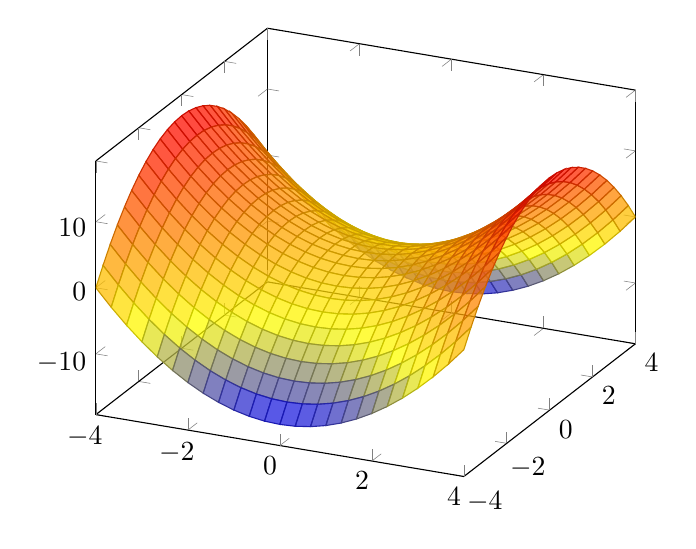
\begin{tikzpicture}
		\begin{axis}[view={25}{30},mark layer=like plot]
			\addplot3 [
				surf,
				shader=faceted,
				fill opacity=0.75,
				samples=25,
				domain=-4:4,
				y domain=-4:4,
				on layer=main,
			] {x^2-y^2};
		\end{axis}
	\end{tikzpicture}
	\caption{An example 3D plot done wit PGFplots.}
\end{figure}

And, of course the code for generating the plot is given as follows:

\begin{code}{latex}
\begin{figure}[!ht]
  \centering
  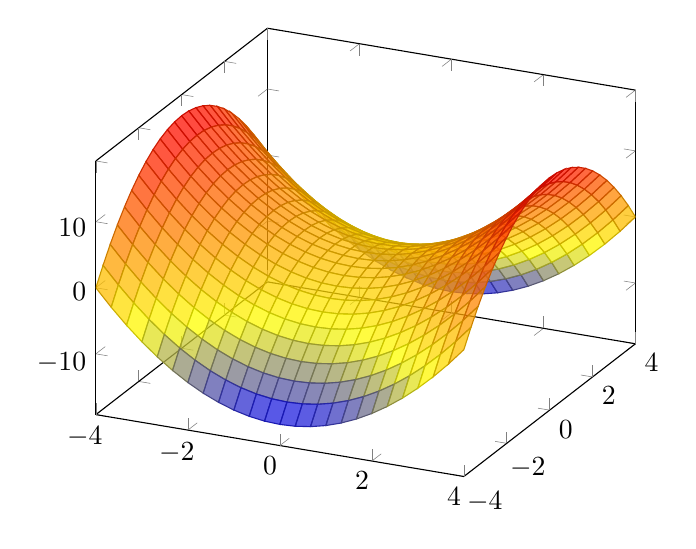
\begin{tikzpicture}
    \begin{axis}[view={25}{30},mark layer=like plot]
      \addplot3 [
      surf,
      shader=faceted,
      fill opacity=0.75,
      samples=25,
      domain=-4:4,
      y domain=-4:4,
      on layer=main,
      ] {x^2-y^2};
    \end{axis}
  \end{tikzpicture}
  \caption{An example 3D plot done wit PGFplots.}
\end{figure}
\end{code}

Some options worth mentioning are as follows:

\begin{hgitemize}
	\item[\pcode{surf}] Generates a \hlight{surface} based on the 2D
	data it was given (in this case these are $x$ and $y$.
	\item[\pcode{shader}] Describes, basically how each segment should be
	filled.
	\item[\pcode{samples}] Similar to 2D plots, tells how many data points will
	be measured. However, make a note that 3D is significantly more taxing
	on the TeX memory than 2D and making this sampling high may result in
	exceeding the memory limit.
\end{hgitemize}

\printbibliography
\end{document}

%%% Local Variables:
%%% coding: utf-8
%%% mode: latex
%%% TeX-command-extra-options: "-shell-escape"
%%% TeX-master: t
%%% TeX-engine: luatex
%%% End:

